\section{EXPERIMENTAL EVALUATION}
\label{sec:experiments}

The experimental evaluation is redesigned around the four security objectives in Section~\ref{subsec-security-objectives}: bounded recovery-belief distortion, bounded false authorization, finite post-attack correction, and bounded deployed-policy deviation. We separate \emph{mechanism-level controlled experiments}, which directly instantiate the update and promotion rules in Sections~V--VI, from \emph{feeder-level recovery experiments}, which require measured power-system/co-simulation traces. This separation is important because the legacy plotting scripts in the repository contain hard-coded draft arrays intended for figure-layout development rather than raw co-simulation logs. Accordingly, the numerical claims reported in this revision are generated only by the reproducible controlled experiments described below; the feeder-level protocol is specified independently and should be populated from measured logs before final submission.

\subsection{Evaluation Questions, Metrics, and Attack Controls}
\label{subsec-exp-questions}

The evaluation addresses four questions. First, does provenance-group capping prevent a bounded number of compromised evidence groups from accumulating unbounded authority in the recovery belief state? Second, after poisoning stops and effective uncompromised evidence becomes aligned again, how quickly does the attacked belief return to the clean reference? Third, does the risk-aware recovery gate keep false authorization below the confidence-budget envelope implied by Theorem~\ref{thm-false-authorization}? Fourth, does stable--candidate separation with a trust-dependent KL radius limit cumulative knowledge-to-policy propagation on the fixed audit distribution used in Section~\ref{subsec-security-objectives}?

We use the same metrics as the formal analysis. Belief integrity is measured by $D_B$ in Eq.~\ref{eq-belief-distance}; action integrity is measured by the false-authorization probability in Eq.~\ref{eq-false-authorization-bound}; correction is measured by $T_{\rm corr}$ in Eq.~\ref{eq-correction-time}; and policy propagation is measured by $D_\pi$ in Eq.~\ref{eq-policy-distance}. For the later feeder-level study, physical recovery should additionally report the weighted restored-service ratio $\eta_t$, time to critical-load restoration, area under the restoration curve (AURC), fallback frequency, verifier calls, and end-to-end decision latency. These physical metrics are secondary to the security objectives: a higher restored-load ratio cannot compensate for false authorization or a violation of the authoritative physical verifier.

\begin{table}[t]
\centering
\caption{Controlled security-experiment configuration.}
\label{tab-exp-controlled-config}
\setlength{\tabcolsep}{1.3mm}
\resizebox{\columnwidth}{!}{
\begin{tabular}{lll}
\toprule[1.3pt]
Experiment & Main controls & Reported quantity \\
\midrule
Belief poisoning &
$\lambda_f=0.85$, $\beta_{\max}=0.025$, $f_p=0{:}5$ &
mean/95th-pct. $D_B$ and Thm.~1 bound \\
Correction &
$f_p=2$, $H_A=2{:}20$, $\epsilon_{\rm corr}=0.02$ &
$T_{\rm corr}$ and Thm.~3 bound \\
Authorization &
$|\mathcal Q(\mathbf a)|=4$, $\epsilon_q=0.005$ &
false-authorization probability \\
Policy promotion &
64 audit states, 4 actions, $K=0{:}10$ &
$D_\pi$ and Thm.~4 bound \\
\bottomrule[1.3pt]
\end{tabular}}
\end{table}

The controlled experiments use a fixed random seed and operate directly on the bounded influence, calibration, and policy-promotion mechanisms. They are not intended to emulate every electrical transient. Their purpose is narrower: to test whether the implemented mechanisms obey the trends and envelopes claimed by the security analysis before they are embedded in the full recovery loop.

\subsection{Recovery-Knowledge Poisoning Scenarios}
\label{subsec-exp-attacks}

The feeder-level attack generator should manipulate evidence rather than directly bypass the trusted actuation path. Table~\ref{tab-exp-attacks} maps the threat model in Section~\ref{subsec-threat-model} to experimental scenarios. Fabrication changes the value of an authenticated assertion; replay and delay preserve a valid identity while changing its temporal relevance; suppression removes supporting or contradicting evidence; correlated-source poisoning compromises several reports that share a provenance root; and outcome-memory poisoning changes the evidence used to qualify later replay transitions. Mixed cases combine one of these knowledge attacks with a physical line, DER, communication, or protection disturbance. Attack intensity is controlled through $\Omega_A=(f_p,B_z,H_A,\epsilon_s)$ rather than through an unqualified percentage of ``malicious data.''

\begin{table*}[t]
\centering
\caption{Recovery-knowledge poisoning scenarios for the feeder-level evaluation.}
\label{tab-exp-attacks}
\setlength{\tabcolsep}{2.0mm}
\resizebox{\textwidth}{!}{
\begin{tabular}{llll}
\toprule[1.3pt]
Attack class & Manipulated recovery evidence & Primary budget control & Primary metrics \\
\midrule
Fact fabrication &
controller availability, measurement trust, protection readiness, outcome status &
$f_p,B_z$ &
$D_B$, false authorization, $\eta_t$ \\
Replay / delay &
stale availability, command-path or measurement-path state &
$H_A,B_z$ &
$D_B$, $T_{\rm corr}$, fallback rate \\
Suppression / missing evidence &
alarm, controller failure, route outage, verified outcome &
$B_z,H_A$ &
uncertainty, fallback rate, recovery delay \\
Correlated provenance poisoning &
multiple reports sharing one compromised upstream component &
$f_p$ &
$D_B$ versus provenance-group cap \\
Outcome-memory poisoning &
post-action success/failure evidence used by replay qualification &
$H_A,B_z$ &
trusted-buffer admission, $D_\pi$ \\
Mixed cyber-physical event &
one knowledge attack plus line/DER/communication/protection disturbance &
$\Omega_A$ &
all four security metrics and physical recovery \\
\bottomrule[1.3pt]
\end{tabular}}
\end{table*}

\subsection{Bounded Belief Distortion and Finite Correction}
\label{subsec-exp-belief}

The first controlled experiment injects bounded differences between attacked and reference provenance groups while keeping uncompromised contributions matched, as required by Theorem~\ref{thm-bounded-poisoning}. For each $f_p$, we run 800 independent 80-update trials. Each compromised group contributes a per-update difference in $[0,2\beta_{\max}]$, reflecting the general case in which a capped group can move from one signed contribution to an opposite signed contribution. Fig.~\ref{fig-exp-belief-budget} reports the maximum belief deviation in each trial together with the analytical envelope.

\begin{figure}[t]
\centering
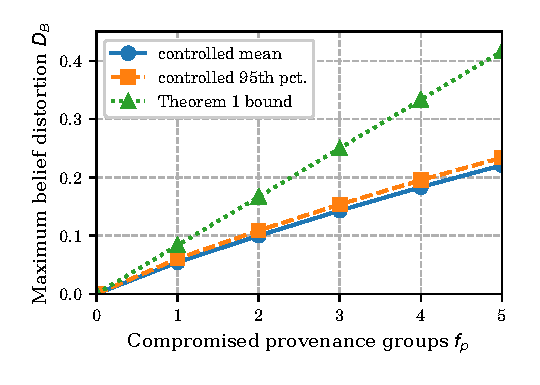
\includegraphics[width=\columnwidth]{figures/kgfedmarl_belief_budget.eps}
\caption{Controlled belief-distortion experiment under increasing numbers of compromised provenance groups. The controlled mean and 95th percentile remain below the sufficient bound from Theorem~\ref{thm-bounded-poisoning}.}
\label{fig-exp-belief-budget}
\end{figure}

The controlled mean $D_B$ increases from 0.0543 at $f_p=1$ to 0.2208 at $f_p=5$, while the corresponding 95th percentiles are 0.0605 and 0.2339. The sufficient bounds are 0.0833 and 0.4167, respectively. The gap is expected because Theorem~\ref{thm-bounded-poisoning} protects against the worst signed difference of every compromised group at every update, whereas the controlled trials sample bounded contributions within that admissible range. The important result is the scaling behavior: the implemented provenance cap keeps the empirical distortion finite and below the budget-dependent envelope as $f_p$ increases.

The correction experiment then applies the worst signed group difference for an attack lasting $H_A$ updates and removes the attack thereafter. The attacked and clean processes receive identical effective uncompromised evidence after $t_a$, matching the sufficient condition in Theorem~\ref{thm-finite-correction}. Fig.~\ref{fig-exp-correction} reports the number of updates required to return within $\epsilon_{\rm corr}=0.02$ of the reference belief.

\begin{figure}[t]
\centering
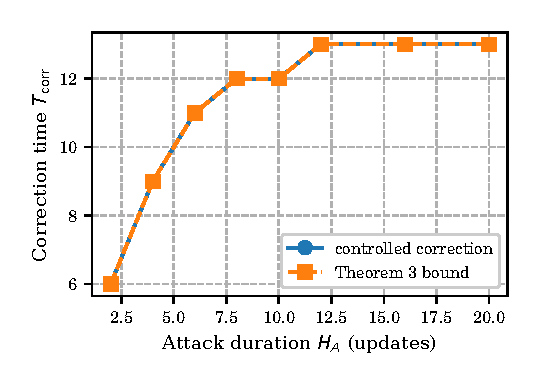
\includegraphics[width=\columnwidth]{figures/kgfedmarl_correction_time.eps}
\caption{Post-attack correction time versus poisoning duration. The controlled recurrence uses the worst per-update signed group difference and therefore follows the sufficient Theorem~\ref{thm-finite-correction} envelope closely.}
\label{fig-exp-correction}
\end{figure}

Correction requires 6 updates after a two-update attack and rises to 13 updates for the longest tested attacks. The curve saturates because the attack-induced log-odds deviation itself is bounded by the geometric accumulation in Eq.~\ref{eq-attack-duration-deviation}. This experiment also clarifies the role of forgetting: $\lambda_f$ is a security parameter, not only a tracking parameter. Increasing it preserves old evidence longer but correspondingly enlarges both the steady poisoning envelope and the post-attack correction time.

\subsection{False Authorization and Policy Propagation}
\label{subsec-exp-auth-policy}

To evaluate the semantic authorization budget, we use actions with four evidence-dependent prerequisites. The controlled belief calibration error is $\epsilon_q=0.005$ per prerequisite, and the aggregate budget $\bar\delta_B$ is swept from 0.01 to 0.10 with equal per-prerequisite allocation. For each point, 200,000 Monte Carlo actions are generated. The independence used by this generator is only an experimental convenience; Theorem~\ref{thm-false-authorization} itself uses a union bound and does not require independent prerequisites.

\begin{figure}[t]
\centering
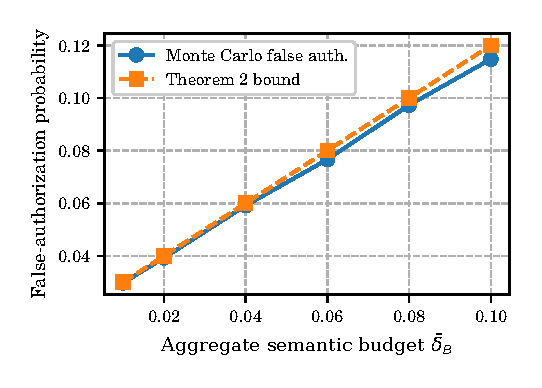
\includegraphics[width=\columnwidth]{figures/kgfedmarl_false_authorization.eps}
\caption{Controlled false-authorization probability under increasing aggregate semantic risk budget. The Monte Carlo rate remains below $\bar\delta_B+\sum_q\epsilon_q$.}
\label{fig-exp-false-auth}
\end{figure}

Across the sweep, the observed false-authorization probability ranges from 0.0297 to 0.1148, while the corresponding sufficient bounds range from 0.03 to 0.12. This experiment tests the calibration-to-authorization link rather than physical feasibility. In the complete recovery loop, a candidate that passes the semantic gate is still subject to the authoritative verifier over $\widehat{\mathcal X}_t$; consequently, the semantic risk budget cannot authorize an invariant physical violation.

The policy-propagation experiment uses 64 fixed audit states and a four-action categorical policy. The attacked and reference deployments start from the same policy and undergo up to ten successful promotion events. Candidate updates are projected to satisfy the trust-dependent KL radii $\kappa_\pi(0.55)=0.00215$ for the lower-trust attacked stream and $\kappa_\pi(0.90)=0.0032$ for the reference stream. Fig.~\ref{fig-exp-policy-drift} compares the resulting audit-distribution TV distance with the cumulative Theorem~\ref{thm-policy-drift} envelope.

\begin{figure}[t]
\centering
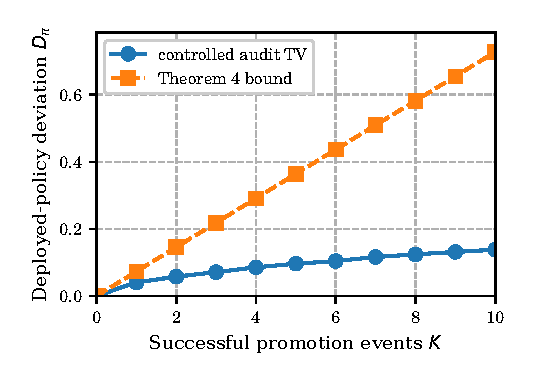
\includegraphics[width=\columnwidth]{figures/kgfedmarl_policy_drift.eps}
\caption{Controlled deployed-policy drift on a fixed audit distribution. The sufficient Theorem~\ref{thm-policy-drift} bound is intentionally conservative because it accumulates worst-case per-promotion TV changes through a triangle inequality.}
\label{fig-exp-policy-drift}
\end{figure}

After ten promotions, the controlled attacked-versus-reference policy deviation is 0.1379, whereas the sufficient cumulative bound is 0.7279. The numerical gap should not be interpreted as looseness that can be removed without stronger assumptions: the theorem deliberately avoids requiring a positive lower bound on every action probability and allows attacked and reference promotion paths to move in different directions at every event. The experiment instead demonstrates that the implemented projection and fixed-audit comparison produce policy changes that remain inside the claimed security envelope.

\subsection{Feeder-Level Recovery Protocol and Ablations}
\label{subsec-exp-feeder}

The final end-to-end study should embed the same evidence manipulation operators in the existing power-system recovery environment and should not replace them with direct policy corruption. The legacy experiment scripts already define IEEE 33-bus, 69-bus, 123-node, and 8500-node recovery layouts and conventional physical/reinforcement-learning baselines; those layouts can be retained, while the old KG/MARL/FL-centric ablations should be replaced by security-boundary ablations that match the revised paper.

The primary end-to-end comparison should include: (i) a physical optimization or rule-based restoration baseline such as MISOCP/FLISR; (ii) a decentralized MARL baseline using the same physical observations but no recovery knowledge plane; (iii) a static-KG MARL baseline that consumes graph features but treats runtime assertions as trusted; and (iv) full KG-FedMARL. The mechanism ablations should disable one trust boundary at a time: \emph{No provenance cap}, \emph{No temporal forgetting}, \emph{No semantic gate}, \emph{No transition quarantine}, and \emph{Fixed promotion radius}. These variants correspond directly to the four security objectives and are more informative for the revised paper than removing generic GAT, asynchronous FL, or personalized adapters.

For each feeder and attack class, the experiment should report mean $\pm$ standard deviation over at least five independent seeds, together with the exact $\Omega_A$, number of evidence sources, number of independent provenance groups, and number of task-critical prerequisites per action. The physical results should be presented jointly with the security metrics. In particular, a method should not be described as better merely because it restores more load if it also raises the false-authorization rate or bypasses the certified fallback more often. The recommended result tuple is
\begin{align}
\big(
\mathrm{AURC},\,
T_{\rm crit},\,
D_B,\,
P_{\rm FA},\,
T_{\rm corr},\,
D_\pi,\,
r_{\rm fb},\,
T_{\rm gate}
\big),
\end{align}
where $r_{\rm fb}$ is the fallback frequency and $T_{\rm gate}$ is the online authorization latency.

\subsection{Reproducibility and Result Provenance}
\label{subsec-exp-repro}

The script \path{figures/Code/kgfedmarl_security_experiments.py} reproduces all numerical curves reported in Figs.~\ref{fig-exp-belief-budget}--\ref{fig-exp-policy-drift} from a fixed seed. It exports vector PDF/EPS files and high-resolution PNG files and can be used as the mechanism-level regression test when the implementation changes. The earlier plotting programs in \texttt{figures/Code} remain useful as layout and baseline templates, but their hard-coded arrays are not treated as measured evidence in this revision. Before final submission, feeder-level figures should be regenerated from archived co-simulation logs or CSV files with seed-level observations, and the manuscript should report only statistics that can be traced back to those files.